\documentclass[a4paper]{article}
\usepackage[utf8]{inputenc}
\usepackage[russian]{babel}
\usepackage[T2]{fontenc}
\usepackage[warn]{mathtext}
\usepackage{graphicx}
\usepackage{amsmath}
\usepackage{floatflt}
\usepackage{amssymb}
\usepackage[left=20mm, top=20mm, right=20mm, bottom=20mm, footskip=10mm]{geometry}


\graphicspath{ {images/} }
\usepackage{multicol}
\setlength{\columnsep}{2cm}


\begin{document}

\begin{titlepage}
	\centering
	\vspace{5cm}
	{\scshape\LARGE Московский физико-технический институт \par}
	\vspace{4cm}
	{\scshape\Large Лабораторная работа \par}
	\vspace{1cm}
	{\huge\bfseries Исследование эффекта Комптона \par}
	\vspace{1cm}
	\vfill
\begin{flushright}
	{\large выполнил студент 653 группы ФФКЭ}\par
	\vspace{0.3cm}
	{\LARGE Веловатый Даниил} \par


\end{flushright}
	

	\vfill

% Bottom of the page
	Долгопрудный, 2018 г.
\end{titlepage}

\section{Цель работы}
\begin{enumerate}
    \item Исследование энергетического спектра $\gamma$-квантов, рассеянных на графите, с помощью сцинтилляционного спектрометра
    \item Определение энергии рассеянных $\gamma$-квантов в зависимости от угла рассеяния
    \item Определение энергии покоя частиц, на которых происходит комптоновское рассеяние
\end{enumerate}

\section{В работе используются:}
\begin{itemize}
    \item источник излучения
    \item графитовая мишень
    \item сцинтилляционный счётчик
    \item ФЭУ
    \item ЭВМ
\end{itemize}

\section{Теоретические положения}
\textbf{Эффект Комптона} - увеличение длины волны рассеянного излучения по сравнению с падающим. Он интерпретируется как результат упругого соударения двух частиц - $\gamma$-кванта и свободного электрона. \par
Пусть электрон до соударения покоился, а  $\gamma$-квант имел начальную энергию \hbar$\omega_0$ и импульс \hbar$\omega_0/c$. После соударения электрон приобретает энергию $\gamma mc^2$, где $\gamma = (1 − \beta^2)^{−1/2}$, $\beta = v/c$, а  $\gamma$-квант рассеивается на некоторый угол $\theta$ по отношению
к первоначальному направлению движения. Энергия и импульс рассеянного излучения — $\propto \omega_1$. Запишем для рассматриваемого процесса законы сохранения энергии и импульса:
\begin{center}
    $mc^2 +$ $\hbar \omega_0 = \gamma mc^2 +$ $\hbar \omega_1$\\
    $\frac{\hbar \omega_0}{c} = \gamma mv \cos \varphi + \frac{\hbar \omega_1}{c} \cos \theta$ \\
    $\gamma mv \sin \varphi = \frac{\hbar \omega_1}{c} \sin \theta$
\end{center}
Решая совместно эти уравнения и переходя от частот к длинам волн, получаем изменение длины рассеянного излучения
\begin{equation}
    \triangle \lambda = \lambda_1 - \lambda_0 = \frac{h}{mc}(1 - \cos \theta) = \Lambda_k(1 - \cos \theta),
\end{equation}
где $\Lambda_k = \frac{h}{mc} = 2.42 \dot 10^{-10}$ см - комптоновская длина волны электрона. \par
Основной целью работы является проверка соотношения (1). Преобразуем его от длин волн к энергии $\gamma$-квантов:
\begin{equation}
    \frac{1}{\varepsilon(\theta)} - \frac{1}{\varepsilon_0} = 1 - \cos \theta,
\end{equation}
где $\varepsilon_0 = E_0/(mc^2)$ - энергия $\gamma$-квантов, падающих на рассеиватель (в единицах $mc^2$), $\varepsilon(\theta)$ - выраженная в тех же единицах энергия квантов, испытавших комптоновское рассеяния на угол $\theta$, $m$ - масса электрона.

\section{Экспериментальная установка}

        \begin{figure}[h]
\begin{center}
\begin{minipage}[h]{0.48\linewidth}
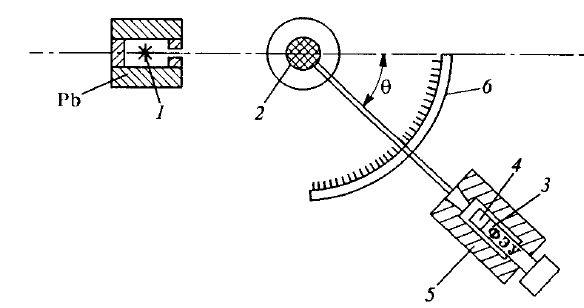
\includegraphics[width=1\linewidth]{fig2.PNG}
\caption{Блок-схема установки по изучению рассеяния $\gamma$-квантов} %% подпись к рисунку\label{ris:experimoriginal} %% метка рисунка для ссылки на него
\end{minipage}
\hfill 
\begin{minipage}[h]{0.48\linewidth}
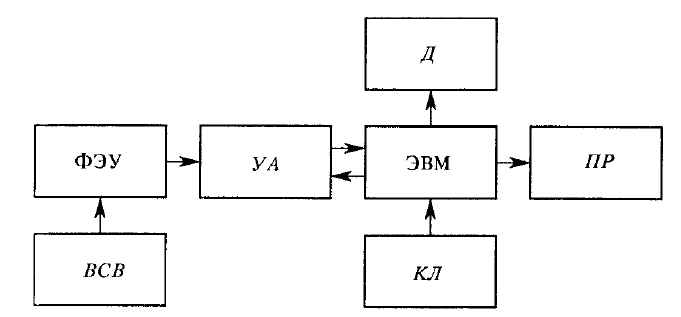
\includegraphics[width=1\linewidth]{fig3.PNG}
\caption{Блок-схема измерительного комплекса}
\label{ris:experimcoded}
\end{minipage}
\end{center}
\end{figure}

Источником излучения служит $^{137}$Cs(1), испускающий  $\gamma$-кванты с энергией 662 кэВ. Узкий пучок после коллиматора попадает на графитовую мишень (2). Кванты, испытавшие комптоновское рассеяния в мишени, регистрируются сцинтилляционным счетчиком и проходят на ФЭУ. Сигналы, возникающие на ФЭУ, подаются на ЭВМ для амплитудного анализа. Штанга с измерительным блоком может вращаться относительно мишени.

\section{Ход работы}

\begin{enumerate}
    \item Подготовим установку к работе. Снимем спектры при углах от 0$^{\circ}$ до 120$^{\circ}$, результаты занесём в таблицу 1.
    
    \item Проведём калибровку прибора, сняв спектры цезия $^{137}$Cs и европия $^{152}$Eu с известными пиками излучения:
    \begin{center}
        $^{137}$Cs: \hspace{1cm} канал 835 \hspace{1cm}	662 кэВ \\
        $^{152}$Eu: \hspace{1cm} канал 479 \hspace{1cm}	341 кэВ \\
        $^{152}$Eu: \hspace{1cm} канал 178 \hspace{1cm}	123 кэВ
    \end{center}
    
    Калибровочный график представлен на рисунке 3.
    
    \begin{figure}[h]
\begin{center}
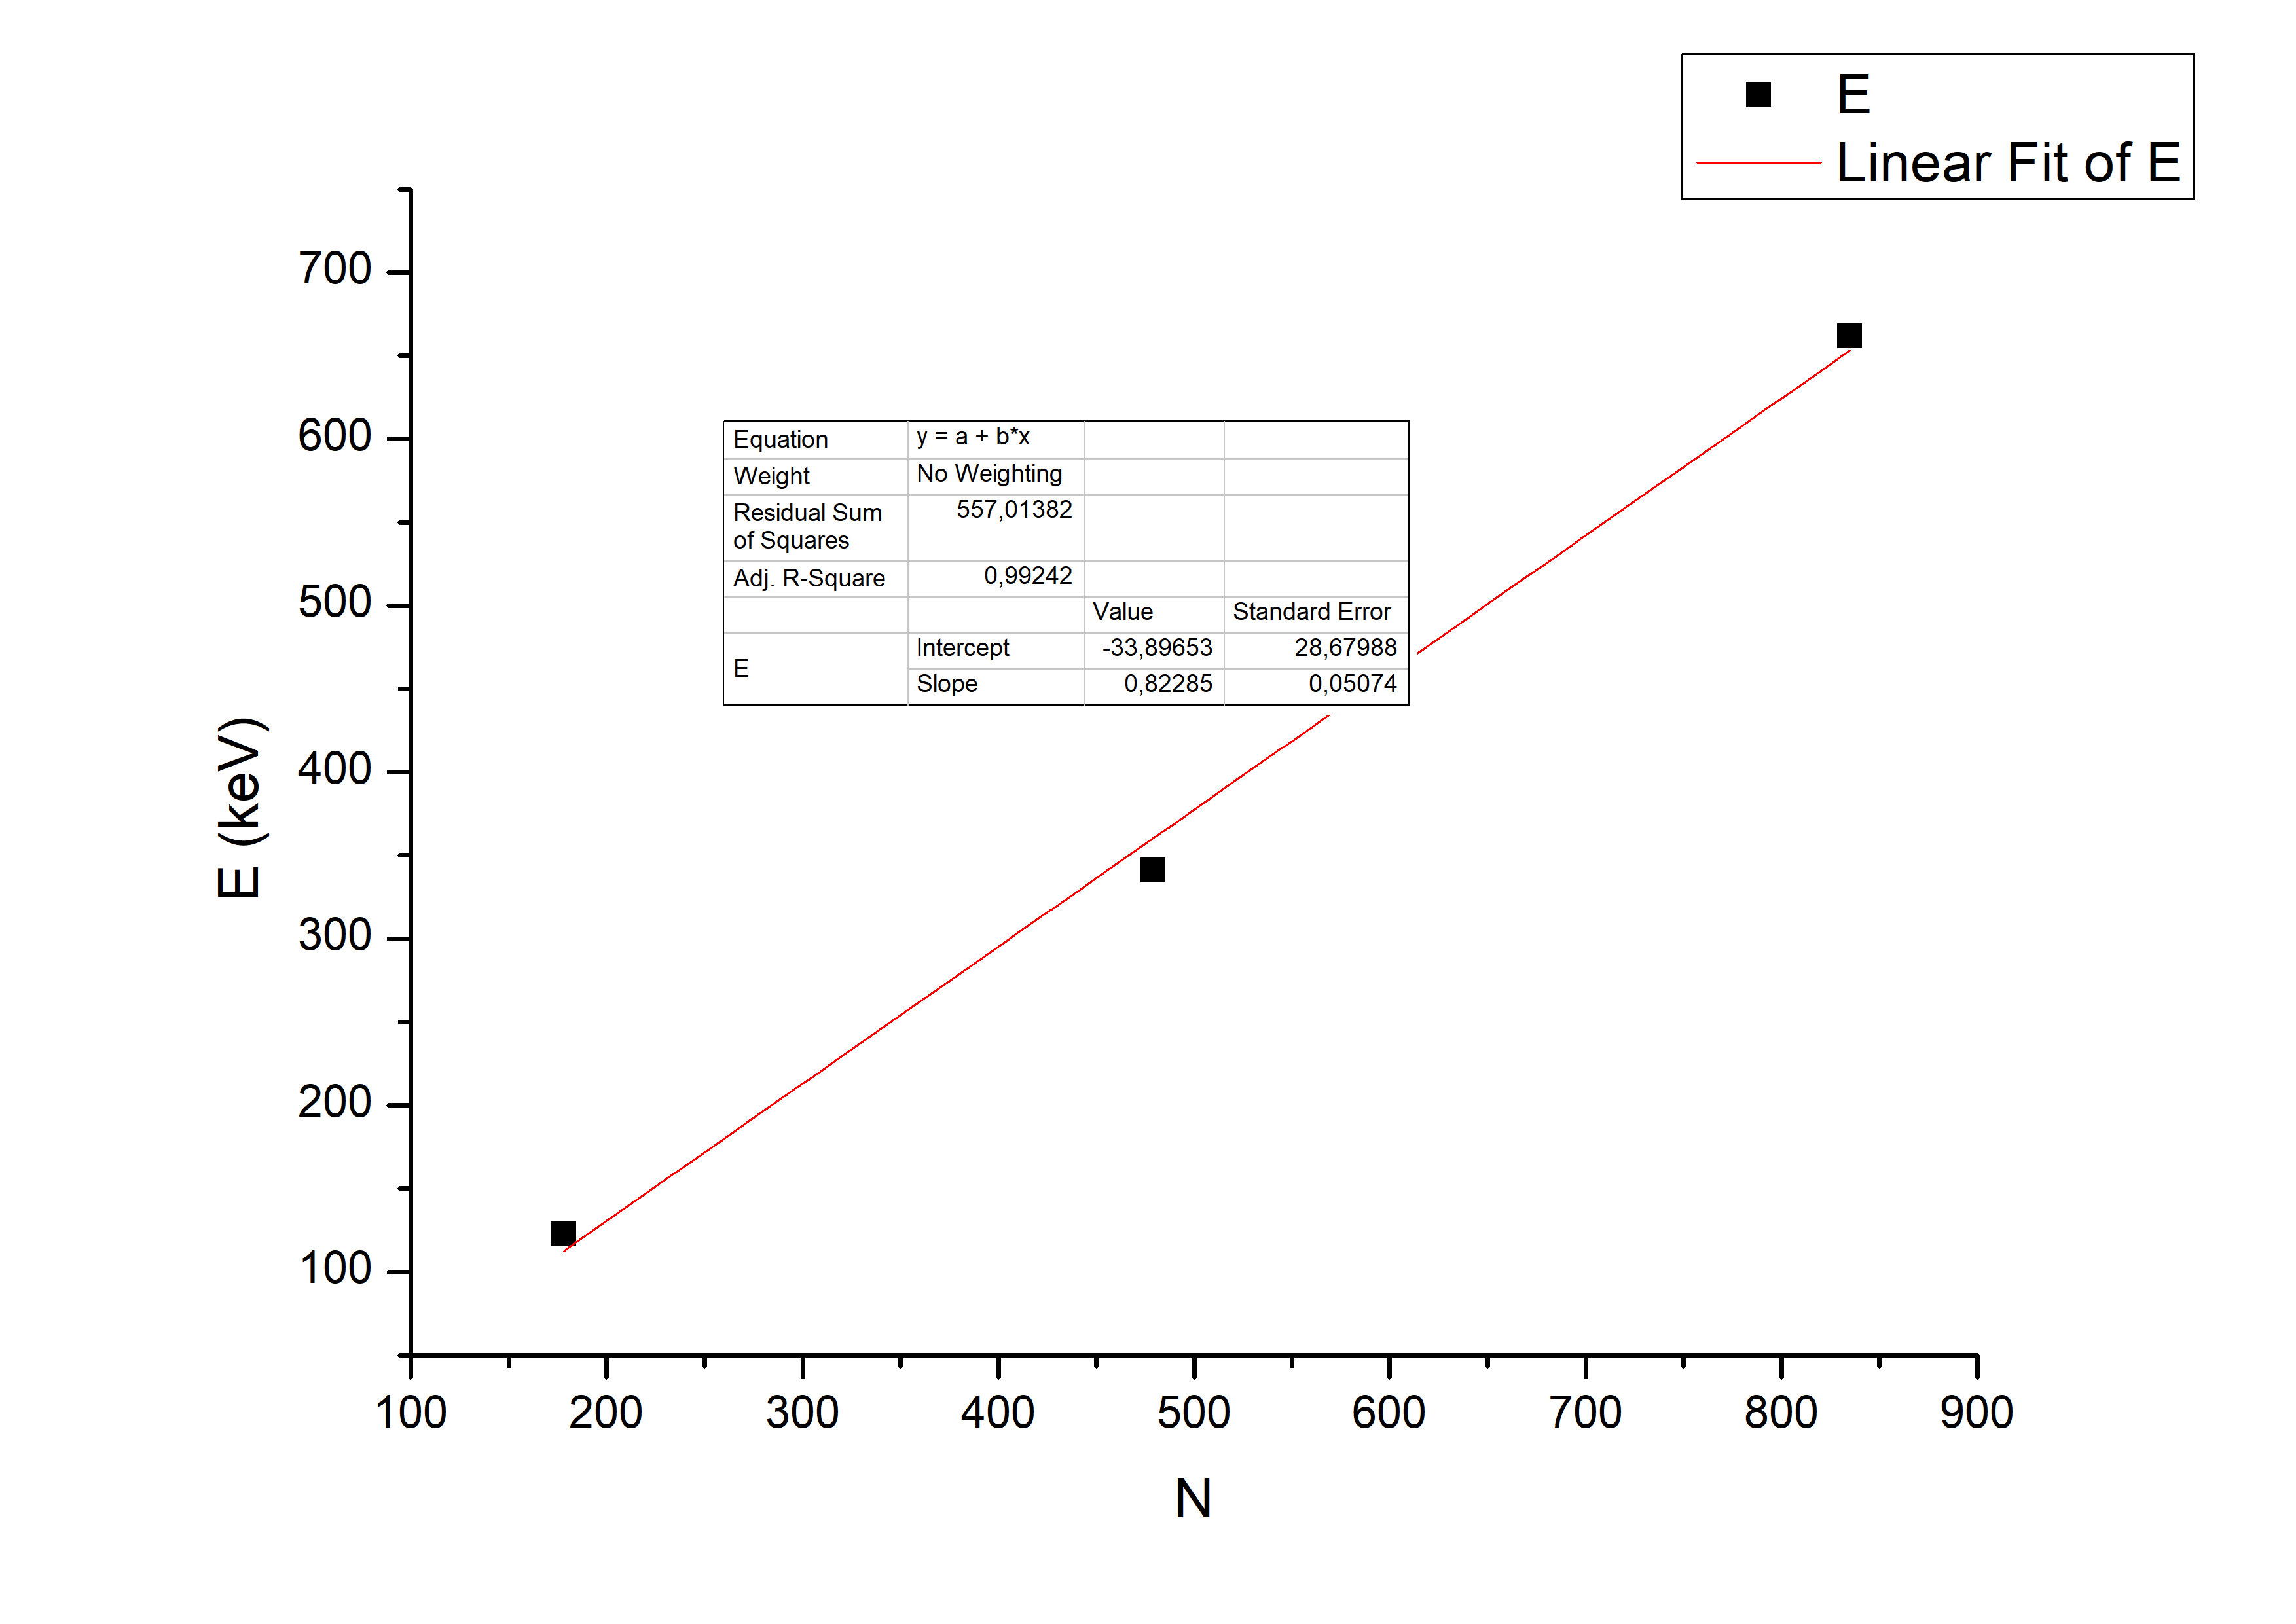
\includegraphics[width=12cm]{Calibration.png}
\caption{Калибровочный график для перехода от номера канала к значению энергии}
\label{ris:experimoriginal} %% метка рисунка для ссылки на него
\end{center}
\end{figure}

    \item В соответствии с калибровочным графиком пересчитаем значения энергии. Построим графики зависимости $1/N = f(1-\cos \theta)$ и $1/E = f(1-\cos \theta)$ (рисунки 4 и 5 соответственно)
    
        \begin{table}[h]
    \centering
    \begin{center}
    \caption{Зависимость номера канала и энергии излучения от угла наблюдения}
    \end{center}
    \vspace{0.1cm}
    \label{tab:my_label}
    \begin{tabular}{|p{1.5cm}||p{0.8cm}|p{0.8cm}|p{0.8cm}|p{0.8cm}|p{0.8cm}|p{0.8cm}|p{0.8cm}|p{0.8cm}|p{0.8cm}|p{0.8cm}|p{0.8cm}|p{0.8cm}|p{0.8cm}|}
\hline
  Угол, $^{\circ}$ & 0 & 10 & 20 & 30 & 40 & 50 & 60 & 70 & 80 & 90  & 100 & 110 & 120 \\
 \hline 
 Номер канала & 941 & 971 & 888 & 735 & 679 & 604 & 522 & 459 & 411 & 365 & 332 & 307 & 302 \\
\hline 
Энергия, кэВ & 806,4 & 833,2 & 759,1 & 622,5 & 572,4 & 505,5 & 432,2 & 376,0 & 333,1 & 292,0 & 262,6 & 240,3 & 235,8
 \\

\hline
 \end{tabular}
\end{table} 
\end{enumerate}

    \begin{figure}[h]
\begin{center}
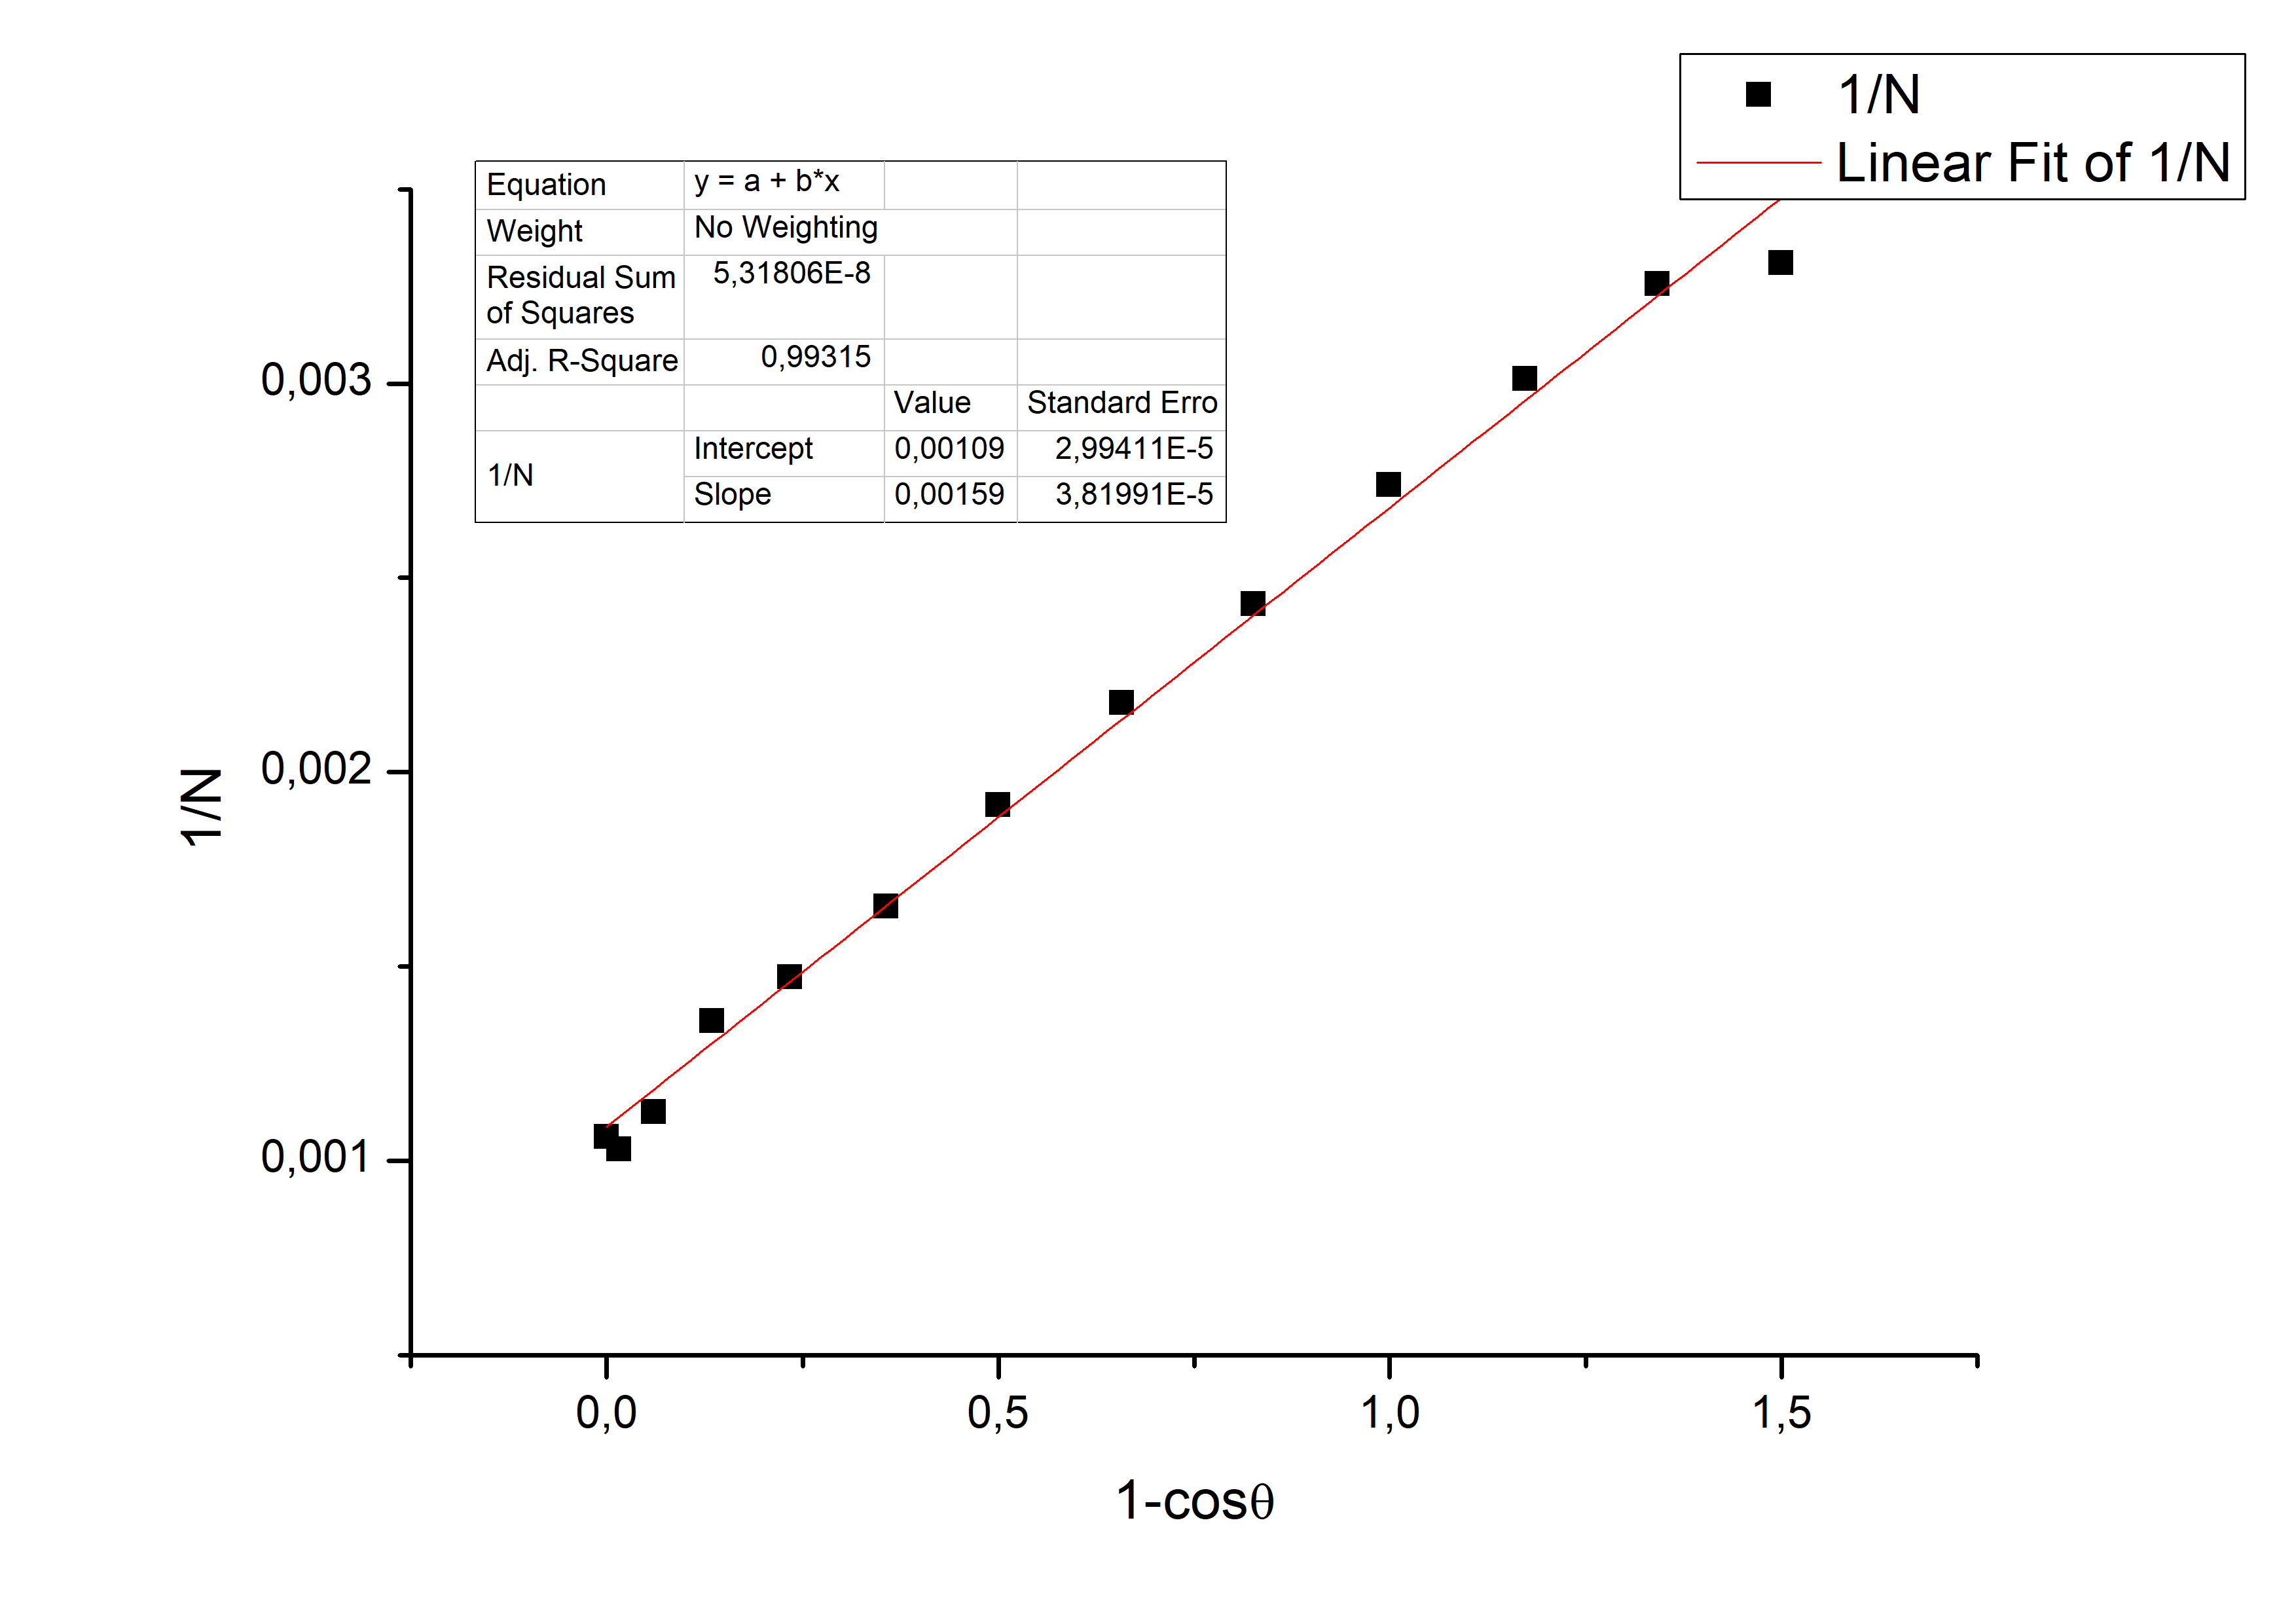
\includegraphics[width=12cm]{N.png}
\caption{График зависимости $1/N = f(1-\cos \theta)$}
\label{ris:experimoriginal} %% метка рисунка для ссылки на него
\end{center}
\end{figure}

    \begin{figure}[h]
\begin{center}
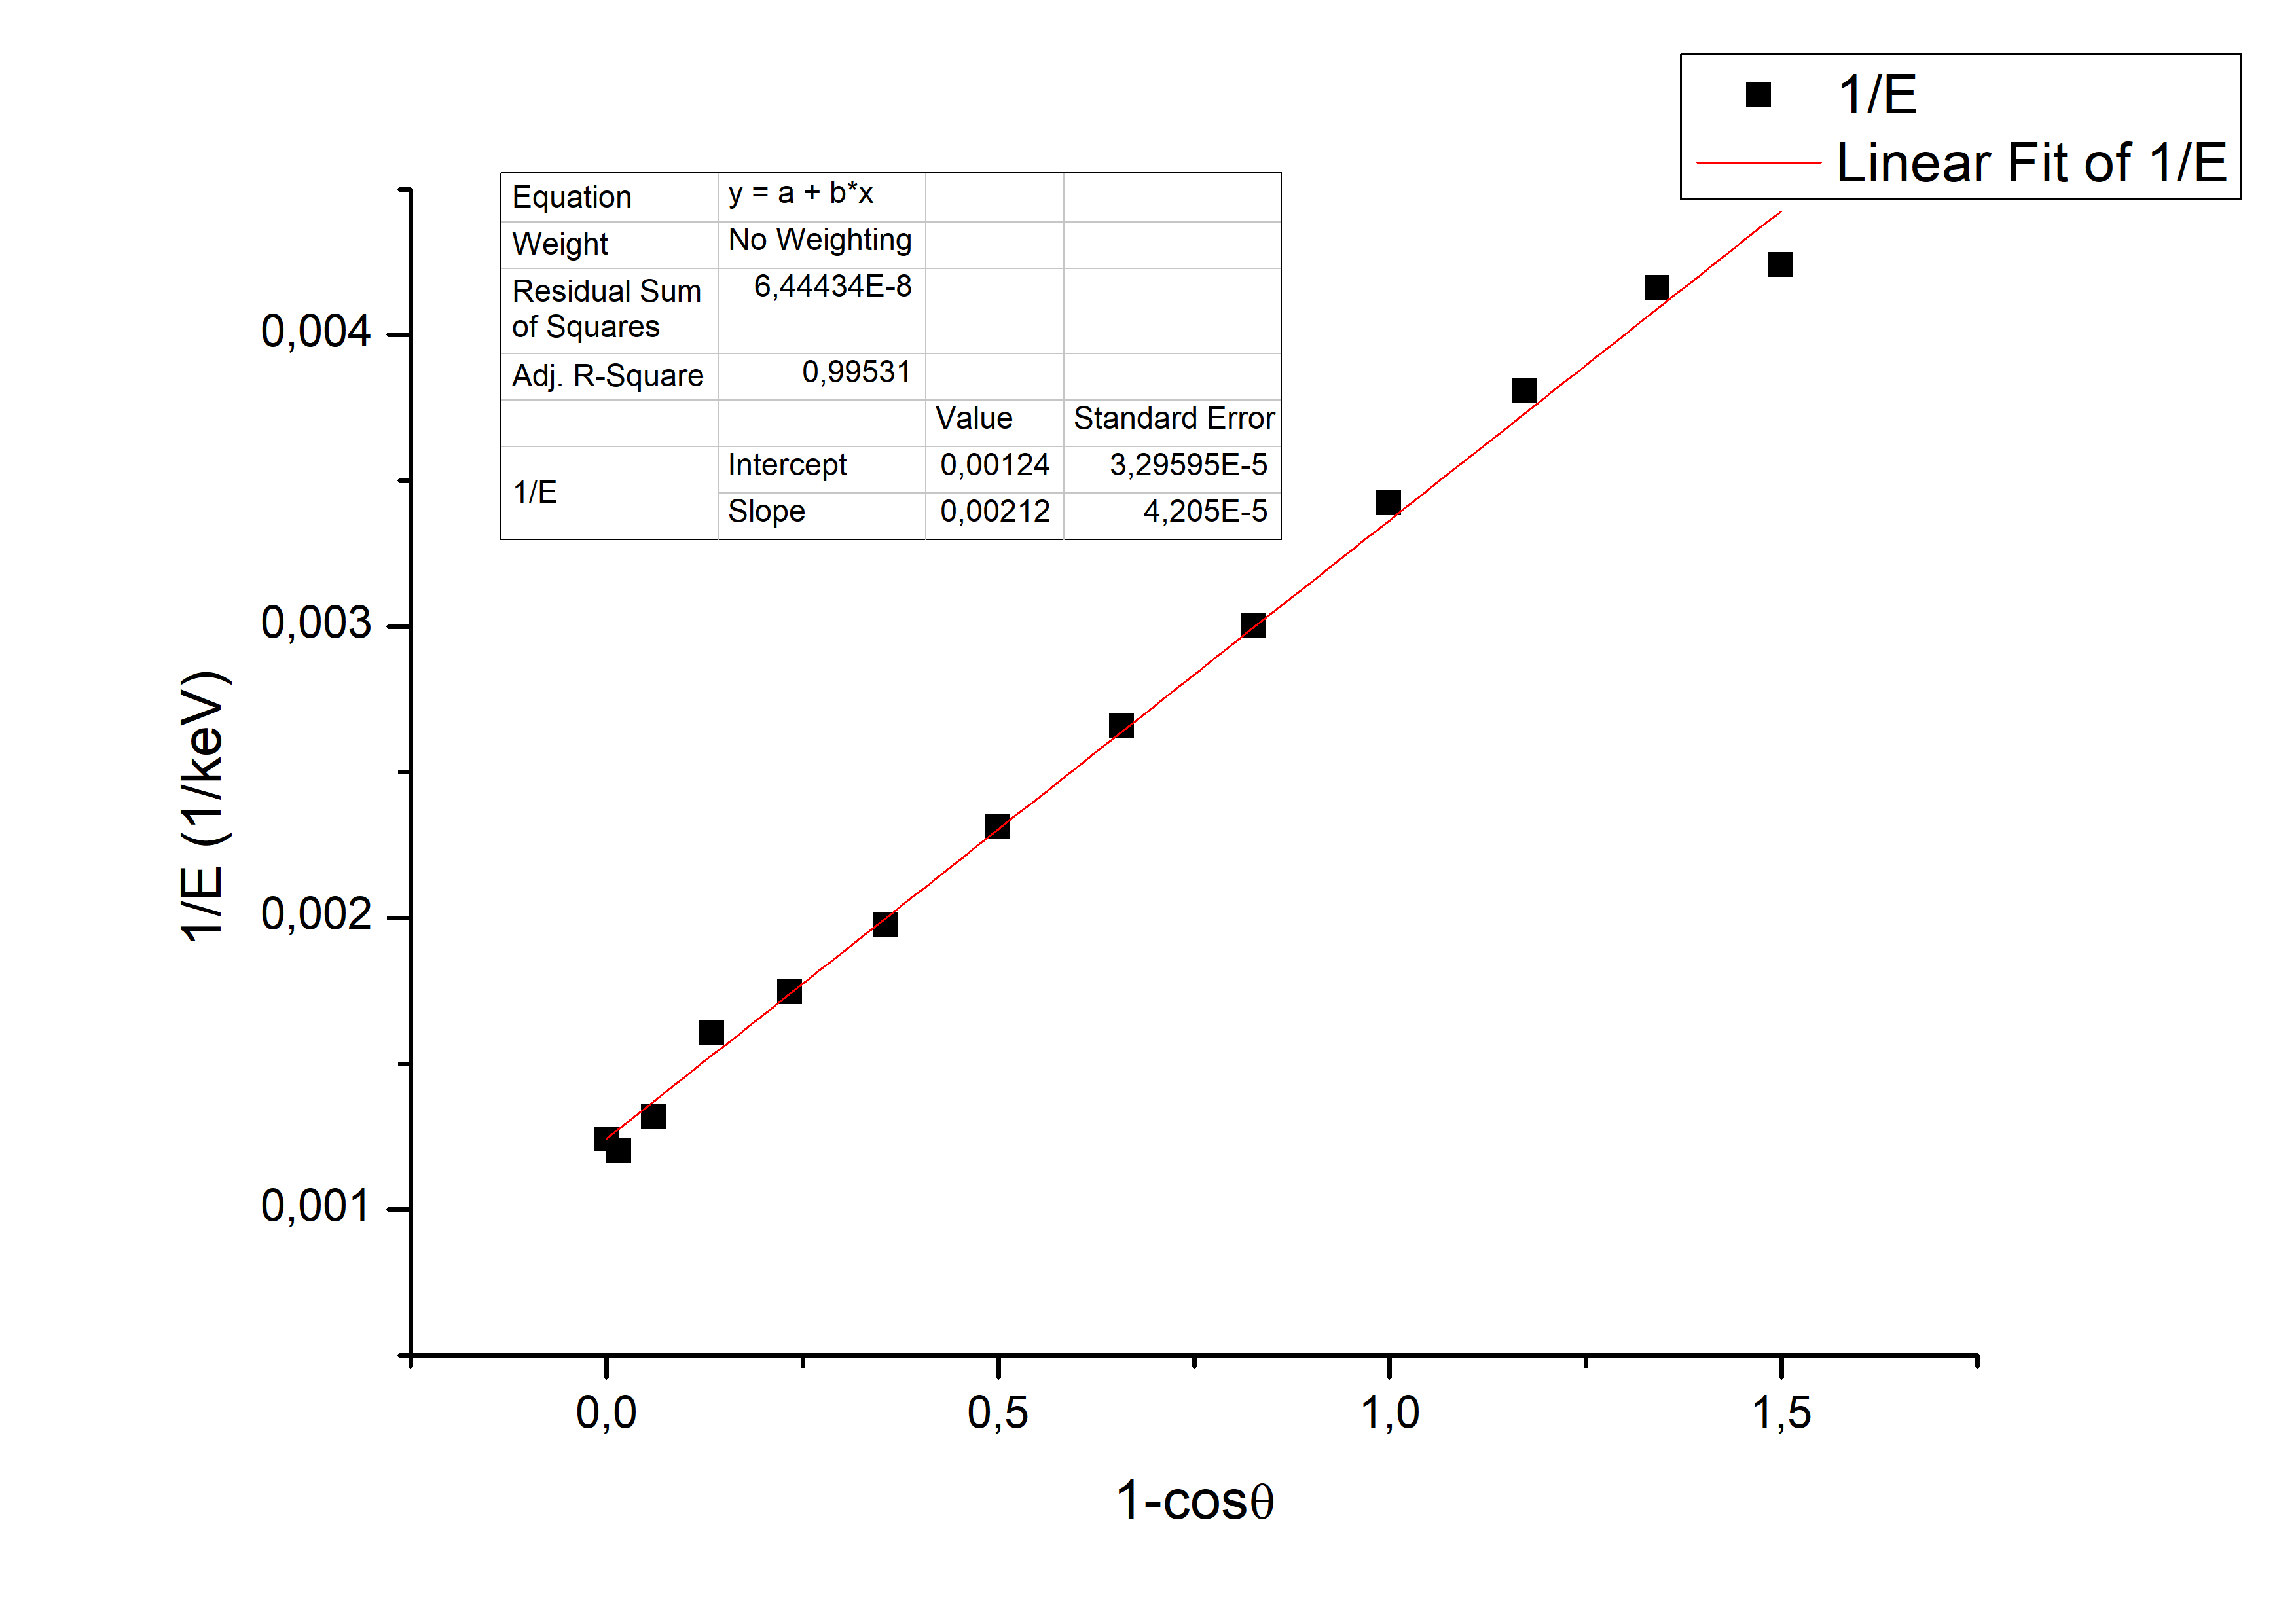
\includegraphics[width=12cm]{E.png}
\caption{График зависимости $1/E = f(1-\cos \theta)$}
\label{ris:experimoriginal} %% метка рисунка для ссылки на него
\end{center}
\end{figure}

\clearpage

\iten Изменим в формуле (2) энергию фотона на номер канала:
\begin{equation}
    \frac{1}{N(\theta)} - \frac{1}{N(0)} = A(1 - \cos \theta)
\end{equation}
С учётом связи между E и N:
\begin{equation}
    mc^2 (\frac{1}{E(90)} - \frac{1}{E(0)}) = 1
\end{equation}
или
\begin{equation}
    mc^2 = E(0) \frac{E(90)}{E(0) - E(90)} = E_{\gamma} \frac{N(90)}{N(0) - N(90)},
\end{equation}
где $E_{\gamma} = 662$ кэВ - энергия налетающего кванта.
Теперь используя графики на рисунках 4 и 5 определим энергию покоя частицы, на которой происходит комптоновское рассеяние. \par
Пересечение прямой с осью ординат определяет $N(0)$ и $E(0)$, с прямой $\cos \theta = 0$ - значение $N(\theta)$ и $E(\theta)$.
\begin{center}
    $N(0) = 917.43$  \hspace{1cm} $N(90) = 373.13$ \\
    $E(0) = 806.45$ кэВ \hspace{1cm} $E(90) = 297.61$ кэВ \\
    \\
    По графику каналов: \\
    \\
    $mc^2 = 662 \frac{373.13}{917.43-373.13}$ = 453.81 кэВ \\
    \\
    По графику энергий: \\
    \\
    $mc^2 = (\frac{1}{297.61} - \frac{1}{806.45})^{-1}$ = 471.68 кэВ
\end{center}

Теоретическое значение энергии покоя электрона составляет 511 кэВ.

\section{Вывод}

В ходе работы был измерен энергетический спектр  $\gamma$-квантов, рассеянных на графите. Экспериментально был проверен эффект Комптона и правильность теоретических соотношений зависимости энергии рассеяния от угла наблюдения. Также в ходе работы была двумя способами (по графику спектров в единицах каналов и по откалиброванному по энергиям графику) определена с хорошей точностью энергия покоя электрона:
\begin{center}
    По каналам: $mc^2 = $453.81 кэВ \\
    По энергиям: $mc^2 = $471.68 кэВ \\
    Теоретическое значение: $mc^2 = $511 кэВ \\
\end{center}
\end{document}
